\firstsection{Introduction}
\maketitle

% (What is the high level motivation)
% What is the obsatcle for effectively apply machine learning model
With the recent advances in neural network based model, machine learning has
gained unprecedented popularity, and its adaption permeated many fields of studies.
%
However, from researchers to practitioners, one often need to overcome many
obstacles during the training, debugging, and tuning processes to unleash
the full potential of these models.
%
Interpreting the internal mechanism and analyzing how predictions are made are critical to both the design and deployment of a given model.
More importantly, the ability to pinpoint where and how an error is made and come up with hypothesis for the cause of failure is the key to identify the limitation and improve upon existing models.
However, providing meaningful answers to these questions are extremely challenging and often regarded as impossible by many.

Recently, substantial research has been developed to combat the model interpretability challenge. Most notably, the works~\cite{} on interpretation of convolution neural network (CNN) model from both machine learning and visualization community has reveal the enormous potential and instant benefits of model interpretation, yet they also remind us how little we actually know regarding the inner mechanism of these deep neural network models. 
%
Many of the existing techniques study the model as an invariant object, where the model's behavior are recorded and analyzed in an offline fashion.
%
However, the exploration natural of these type of analysis often lead to \emph{what if ...} types of questions. What if I perturbed the current input? Will the prediction be stable? What if when change the internal state of the model, how could the change affect the prediction. What if the current prediction is wrong, how and where should we change the model in order to produce the correct result? These type of dynamic queries is a natural way for us to gain understanding and come up with hypothesis of the model mechanisms by \emph{interrogating} the relationship between the input, internal states, and output prediction. Yet we do not often need to setup extra specialized experiment to answer.

Compare to image classification task, natural language processing systems have a number of innate restriction (e.g., the discrete nature of words) that makes interpreting them even more challenging. For example, \emph{feature visualization}~\cite{}, an often deployed technique for illustrating what kind of image feature a given part of the network (e.g., neuron, layer, or channel) captures, can not be easily generalized and applied for natural language due to the requirement of a continuous solution space (i.e., the image pixel values). Even though we can encode a word as an vector~\cite{}, the word embedding space is still a discretely defined space, where the interpolation between two vectors (i.e., two words) do not corresponds to explicit meaning.

On the one hand, recognize where the model fail is non-trivial. The standard evaluation approach (i.e., the prediction accuracy on the test set) provides limited information and cannot answer many important questions (e.g., how stable the prediction is, which part of the model may contribute to the failure) that are essential to the model diagnostic process. On the other hand, infer the cause of model failure is even more challenging. Neural network models are often referred to as black boxes due to the hard to recognize  difficult to interpret parameter, hypothesizing what happened in prediction process require the ability to peek inside the model and understand the intricate relationships among model inputs, critical internal mechanisms, as well the output predictions.

%\begin{itemize}
%    \item Study the classifier  vs. single instance evaluation
%    \item Model agnostic vs. reveal internal states
%    \item View model as invariant object vs. interrogate the model via partial/full updates
%\end{itemize}

Questions such as, how stable predictions are concerning small perturbation in the input, how are these predictions arrived (i.e., the model may come up with the correct prediction by pickup unintended feature/alignment), and what are the often made mistakes, are all essential in systematic examination and evaluation of the model. 
%%%%%%%%% accessing internal states are important %%%%%%%%%%%%



% Making sense and explaining predictions made by neural networks is also becoming a necessity.
%
Many works~\cite{RibeiroSinghGuestrin2016} have been dedicated to providing intuitive explanations for a given prediction, several of which approach the problem from a model agnostic approach that made them applicable to different applications (i.e., by fitting a simplier linear model near the prediction of interests).
%
Despite being invaluable for the providing human understandable explaination, the lack of the ability to access and explore the internal states of the model, which is vitally important to make sense of why a model fail, limits their ability for more in depth exploration and evaluation of the model.


%%%%%%%%%% interrogate relationship between different components, modified different components %%%%%%%%%%%
Beside looking into the internal states, understanding how each of the component of the model interact with input and output as well as with each other is the crucial for truly exmaine the mechanism of the model.
%
Look at how the model work in action and interrogate relationship between different component, i.e., how the change made to one part of model affect the other pieces present, is the key to gain the full picture.

\begin{figure}[htbp]
\centering
\vspace{-2mm}
 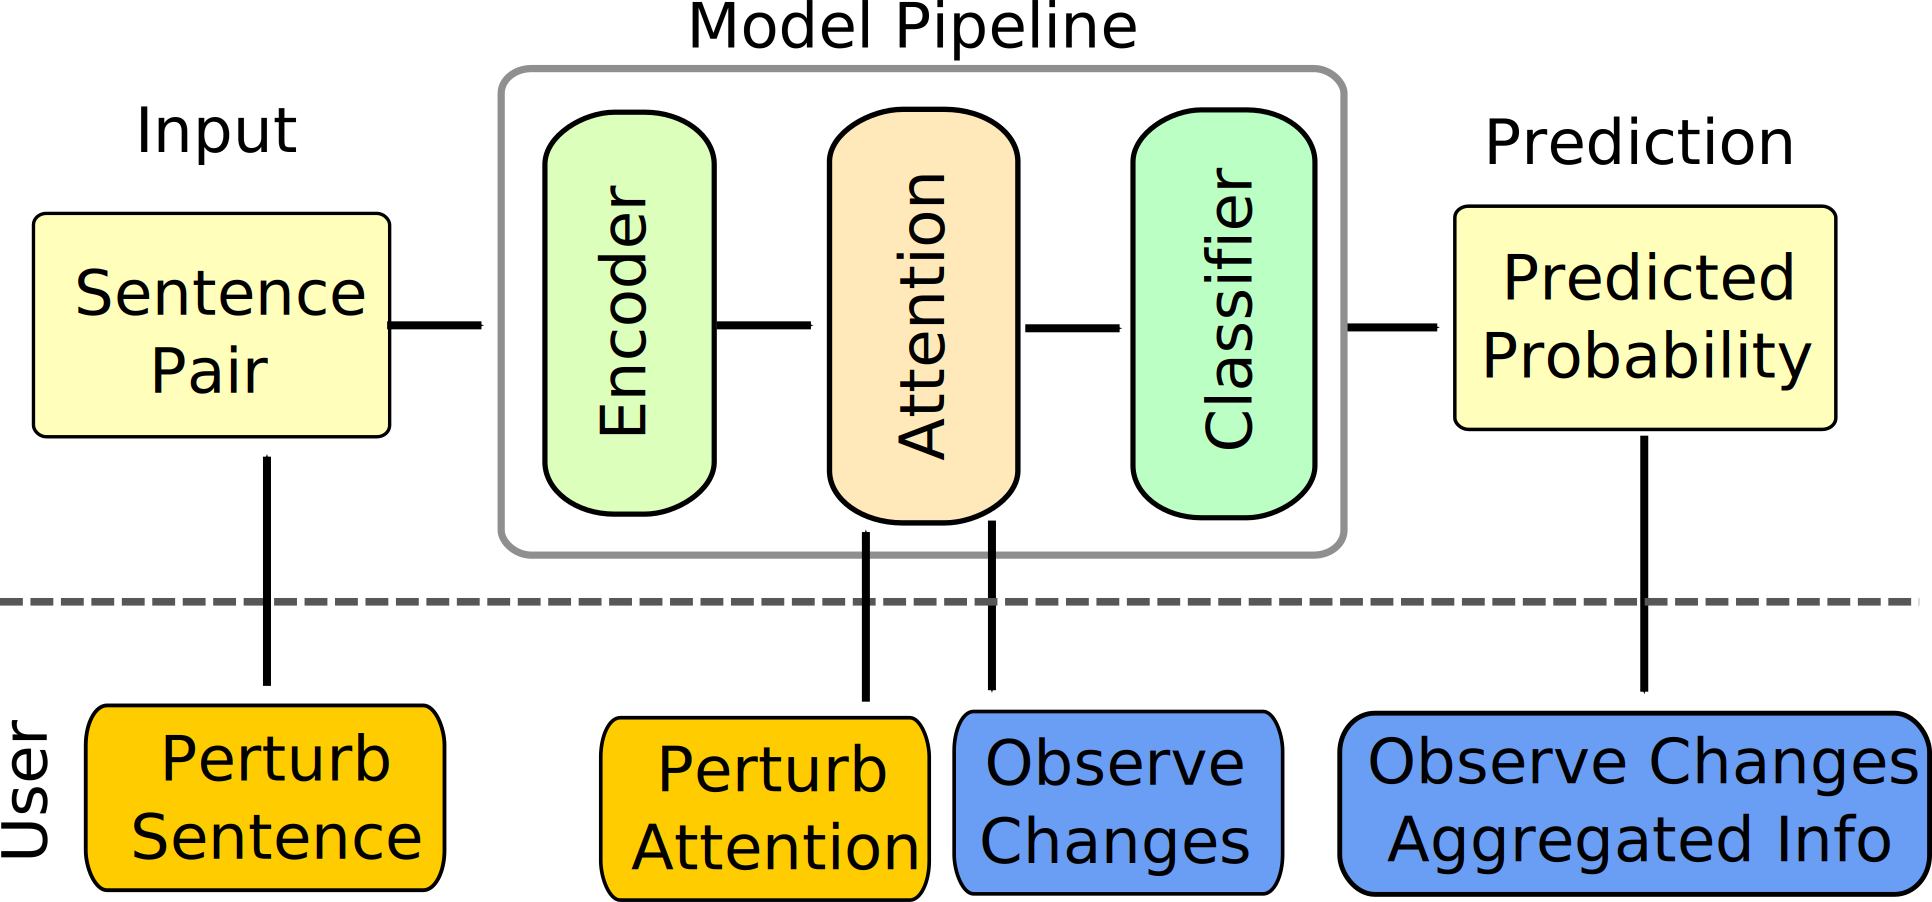
\includegraphics[width=1.0\linewidth]{pipeline}
 \caption{Language Inference Model Pipeline.}
\label{fig:projTransition}
\end{figure}

In this work, we introduce a visualization system that through a tight yet flexible integration between visual analytic elements and the underlying model, allow a user to interrogate the model by perturbing the input, the internal state, as well as prediction while observing changes in other parts of the pipeline.
We use natural language inference task~\cite{BowmanAngeliPotts2015} as an example to illustrate how this system help natural language processing (NLP) researchers quickly identify the potential limitation of an NLP model, probe the inner states of the model for interpreting key mechanism such as attention, and ultimately come up with hypothesis on why the model fails.

% ######## Why use perturbation ###########
% Iterate the model design and debug the system hinged on the ability to quickly
% identify the errors made by a model.
%
% Perturbe the input is what NLP researchers have subconsciously been doing to study and test a model.
%
% Interpret/probe the relationship between attention and the prediction result


The key contributions of the proposed works is summarized as the following:
\begin{itemize}
    \item Identify the mistakes made by the model through perturbation of input sentences and visual summarization of the predictions;

    \item Enhance the visual representation of attention by overlaying sentence linguistic structure to allow grammar guided simplification;

    \item Enable the interrogation of the relationship between input sentences, attention, and the prediction by interactively exploring how the change in one of these elements affect other parts of the model.

\end{itemize}
